\section{Polar Coordinates}
\begin{itemize}
    \item In polar coordinates, we can represent polar coordinates in terms of the distance $r$ from the origin and the angle it makes with the positive horizontal axis:
    \begin{equation}
        (x,y) \iff [r,\theta]
    \end{equation}
    \item The magnitude of $r$ gives the distance from the origin, and multiplying $r$ by $-1$ rotates the point about the origin by $\pi$.
    \item Polar coordinates are not unique:
    \begin{itemize}
        \item The pole is $[0,\theta]$ for all $\theta$.
        \item $[r, \theta] = [r ,\theta + 2n\pi]$ for any integer $n$.
        \item $[r,\theta] = [-r, \theta + (2n+1)\pi]$ for any integer $n$.
    \end{itemize}
    \item We can convert between cartesian and polar coordinates using the transformation:
    \begin{align}
        x &= r\cos\theta \\ 
        y &= r\sin\theta
    \end{align}
    which gives:
    \begin{align}
        r &= \sqrt{x^2+y^2} \\ 
        \theta &= \arctan\left(\frac{y}{x}\right)
    \end{align}
    for $x\neq 0$.
    \begin{example}
        Suppose we have the following four points.
        \begin{center}
            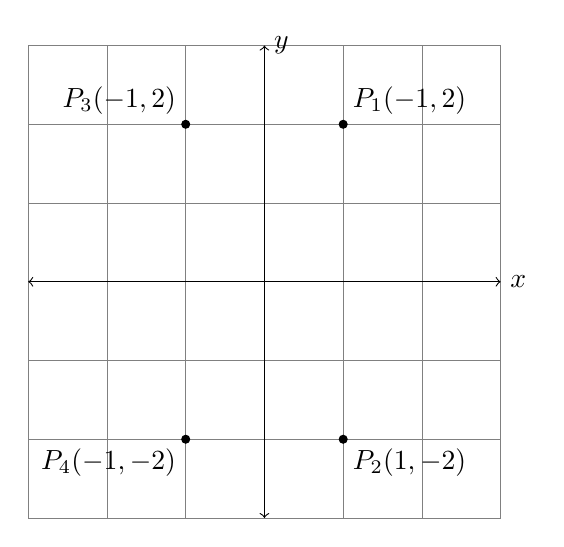
\begin{tikzpicture}
                \draw[step=1,gray,very thin] (-3,-3) grid (3,3);
                \draw[fill=black] (1,2) circle (0.05) node[above right] {$P_1(-1,2)$};
                \draw[fill=black] (1,-2) circle (0.05) node[below right] {$P_2(1,-2)$};
                \draw[fill=black] (-1,2) circle (0.05) node[above left] {$P_3(-1,2)$};
                \draw[fill=black] (-1,-2) circle (0.05) node[below left] {$P_4(-1,-2)$};
                \draw[<->] (-3,0) -- (3,0) node[right]{$x$};
                \draw[<->] (0,-3) -- (0,3) node[right]{$y$};

                \end{tikzpicture}
        \end{center}
        We can represent the four coordinates also as:
        \begin{align}
            P_1[\sqrt{5}, 1.107] \\ 
            P_2[\sqrt{5}, -1.107] \\ 
            P_3[-\sqrt{5}, -1.107] \\ 
            P_4[-\sqrt{5}, 1.107]
        \end{align}
    \end{example}
    \item We can represent straight lines as:
    \begin{itemize}
        \item Straight lines: $y=mx$: $r=\alpha$ with $\alpha=\arctan(m)$.
        \item Vertical lines $x=a$: We have $r\cos\theta = a \implies r = a\sec\theta$.
        \item Horizontal lines: $y=b$. We have $r\sin\theta=b \implies r=b\csc\theta$
    \end{itemize}
    \item We can represent circles in polar coordinates as:
    \begin{equation}
        x^2 + y^2 = 9 \iff r = 3
    \end{equation}
    \item Converting \textit{from} polar coordinates requires a bit of extra work. Suppose we have $r=6\sin\theta$, then:
    \begin{align}
        r^2 &= 6r\sin\theta \\ 
        x^2+y^2 &= 6y \\ 
        x^2+y^2-6y+9=9 \\ 
        x^2 + (y-3)^2 &= 9
    \end{align}
    which represents a circle with radius $3$ centered at $(0,3)$.
    \item Symmetry can also arise in many scenarios. For example:
    \begin{itemize}
        \item Symmetry about $x$ axis: $[r_1,\theta]$ and $[r_1, -\theta]$.
        \item Symmetry about $y$ axis: $[r, \pi-\theta]$ and $[r_1, \theta]$.
        \item Symmetry about origin: $[r,\theta]$ and $[r, \theta + \pi]$.
    \end{itemize}
    which will help when sketching them.
    \begin{example}
        Suppose we wish to sketch the curve $r= \frac{1}{2} + \cos\theta$. Notice that this is periodic so we only need to look at values of $\theta$ where $0 \le \theta < 2\pi$.
        \begin{enumerate}
            \item Let us first find values of $\theta$ (if possible) that make $r=0$:
            \begin{equation}
                0 = \frac{1}{2} + \cos\theta \implies \theta = \frac{2\pi}{3}, \frac{4\pi}{3}
            \end{equation}
            \item Find local max and min values of $r$:
            \begin{equation}
                \frac{dr}{d\theta} = -\sin\theta = 0 \implies \theta = 0, \pi
            \end{equation}
            At $\theta=0$, we have $r=\frac{3}{2}$, at $\theta= \pi$ we have $r = -\frac{1}{2}$. If $\theta = \frac{\pi}{2}, \frac{3\pi}{2}$, then $r=\frac{1}{2}$.
            \item We then loko at symmetry. Notice that:
            \begin{equation}
                \frac{1}{2} + \cos(-\theta) + \frac{1}{2}+\cos\theta
            \end{equation}
            However:
            \begin{align}
                r(\theta - \pi) \neq r(\theta) \\ 
                r(\pi + \theta) \neq r(\theta)
            \end{align}
            so it is not symmetryic about the $y$ axis or origin.
            \item We now look at the relevant intervals. From $0 \le \theta < \frac{2\pi}{3}$, we have $\frac{dr}{d\theta} < 0$ so the radius is monotonically decreasing.
            \vspace{2mm}

            We can also look at the interval $\frac{2\pi}{3} \le \theta < \pi$ and see that $r$ is negative and $\frac{dr}{d\theta} < 0$, so the manigutde of $r$ \textit{increases}.
            \vspace{2mm}

            Noting that the function is differentiable at $\theta=\pi$, we can reflect the shape about the $x$ axis to get a Limacon with inner loop.
        \end{enumerate}
    
    \begin{center}
        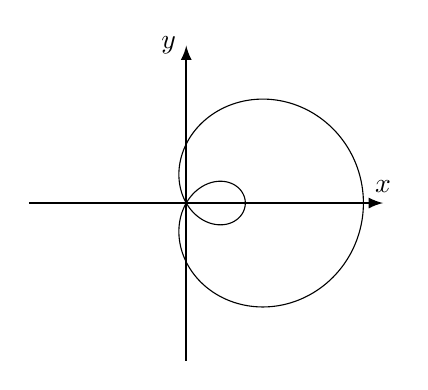
\begin{tikzpicture}
            \draw[thick,->,>=latex] (-2,0)--(2.5,0) node[above] {$x$};
            \draw[thick,->,>=latex] (0,-2)--(0,2) node[left] {$y$};
            \draw[domain=0:540,scale=1.5,samples=500] plot (\x:{0.5+cos(\x)});
        \end{tikzpicture}
    \end{center}
    \end{example}
    \item There are a few common shapes. Each of these could be flipped or rotated by shifting the argument $\theta$, or using negative numbers.
    \begin{itemize}
        \item Circles:
        \begin{equation}
            r = -2\cos\theta
        \end{equation}
        \begin{center}
            \begin{tikzpicture}
                \draw[thick,->,>=latex] (-3,0)--(3,0) node[above] {$x$};
                \draw[thick,->,>=latex] (0,-3)--(0,3) node[left] {$y$};
                \draw[domain=0:540,scale=1.5,samples=500] plot (\x:{-2*cos(\x)});
            \end{tikzpicture}
        \end{center}
        \item Cardioids:
        \begin{equation}
            r= a + a\cos\theta 
        \end{equation}

        \begin{center}
            \begin{tikzpicture}
                \draw[thick,->,>=latex] (-3,0)--(3,0) node[above] {$x$};
                \draw[thick,->,>=latex] (0,-3)--(0,3) node[left] {$y$};
                \draw[domain=0:540,scale=1.5,samples=500] plot (\x:{1+1*cos(\x)});
            \end{tikzpicture}
        \end{center}
        \item Limacons:
        \begin{equation}
            r=a+b\sin\theta
        \end{equation}
        There are two types, for $a>b$:
        \begin{center}
            \begin{tikzpicture}
                \draw[thick,->,>=latex] (-3,0)--(3,0) node[above] {$x$};
                \draw[thick,->,>=latex] (0,-3)--(0,3) node[left] {$y$};
                \draw[domain=0:540,scale=1.5,samples=500] plot (\x:{1+0.5*cos(\x)});
            \end{tikzpicture}
        \end{center}
        For $a<b$:
        \begin{center}
            \begin{tikzpicture}
                \draw[thick,->,>=latex] (-3,0)--(3,0) node[above] {$x$};
                \draw[thick,->,>=latex] (0,-3)--(0,3) node[left] {$y$};
                \draw[domain=0:540,scale=1.5,samples=500] plot (\x:{0.5+1*cos(\x)});
            \end{tikzpicture}
        \end{center}
        \item Leminiscates. Again, there are two types. For:
        \begin{equation}
            r^2 = a\sin(2\theta)
        \end{equation}
        \begin{center}
            \begin{tikzpicture}
                \draw[thick,->,>=latex] (-3,0)--(3,0) node[above] {$x$};
                \draw[thick,->,>=latex] (0,-3)--(0,3) node[left] {$y$};
                \draw[domain=0:90,scale=1.5,samples=500] plot (\x:{sqrt(sin(2*\x))});
                \draw[domain=0:90,scale=1.5,samples=500] plot (\x:{-sqrt(sin(2*\x))});
            \end{tikzpicture}
        \end{center}
        and:
        \begin{equation}
            r^2 = a\cos(2\theta)
        \end{equation}
        \begin{center}
            \begin{tikzpicture}
                \draw[thick,->,>=latex] (-3,0)--(3,0) node[above] {$x$};
                \draw[thick,->,>=latex] (0,-3)--(0,3) node[left] {$y$};
                \draw[domain=-45:45,scale=1.5,samples=500] plot (\x:{sqrt(cos(2*\x))});
                \draw[domain=-45:45,scale=1.5,samples=500] plot (\x:{-sqrt(cos(2*\x))});
            \end{tikzpicture}
        \end{center}
        \item Petal curves:
        \begin{align}
            r &= a\sin(n\theta) \\ 
            r &= a\cos(n\theta)
        \end{align}
        where $n$ is an integer. There are $n$ petals if $n$ is odd and $2n$ petals if $n$ is even. For example, the following is: $r=2\cos 3\theta$:
        \begin{center}
            \begin{tikzpicture}
                \draw[thick,->,>=latex] (-3,0)--(3,0) node[above] {$x$};
                \draw[thick,->,>=latex] (0,-3)--(0,3) node[left] {$y$};
                \draw[domain=0:360,scale=1.5,samples=500] plot (\x:{2*cos(3*\x)});
            \end{tikzpicture}
        \end{center}
        and for $r=2\sin(4\theta)$:
        \begin{center}
            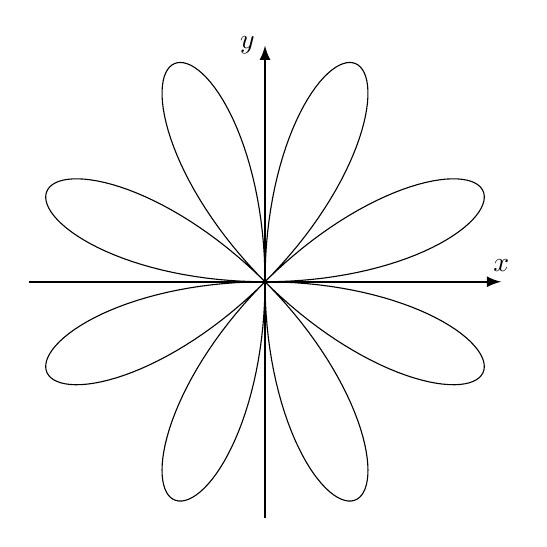
\begin{tikzpicture}
                \draw[thick,->,>=latex] (-3,0)--(3,0) node[above] {$x$};
                \draw[thick,->,>=latex] (0,-3)--(0,3) node[left] {$y$};
                \draw[domain=0:360,scale=1.5,samples=500] plot (\x:{2*sin(4*\x)});
            \end{tikzpicture}
        \end{center}
    \end{itemize}
    \item We can also find the intersection of polar coordinates, but we have to be careful. The following example illustrates why.
    \begin{example}
        Suppose we have two curves $r=\sin\theta$ and $r=-\cos\theta$. Suppose we try to solve this via:
        \begin{equation}
            \sin\theta = -\cos\theta \implies \theta = \frac{3\pi}{4}, \frac{7\pi}{4}
        \end{equation}
        Plugging this back into $x=r\cos\theta$ and $y=r\sin\theta$, we get $x=-\frac{1}{2}$ and $y=-\frac{1}{2}$. We can also use $\theta=\frac{7\pi}{4}$ to get: $x=-\frac{1}{2}$ and $y=\frac{1}{2}$ which is the same point. However, it represents the curves below:
        \begin{center}
            \begin{tikzpicture}
                \draw[thick,->,>=latex] (-3,0)--(3,0) node[above] {$x$};
                \draw[thick,->,>=latex] (0,-3)--(0,3) node[left] {$y$};
                \draw[domain=0:540,scale=1.5,samples=500] plot (\x:{-cos(\x)});
                \draw[domain=0:540,scale=1.5,samples=500] plot (\x:{sin(\x)});
            \end{tikzpicture}
        \end{center}
        There is actually two intersection points! The reason for this is that we assumed that the two curves intersect at the same value of $\theta$, but this is not necessarily true for the origin, which can be obtained at any angle $\theta$.
    \end{example}
    \item As a result, we also have to check the origin.
    \item It is also possible to find the tangent:
    \begin{align}
        \frac{dy}{dx} &= \frac{
            \frac{dy}{d\theta}
            }{
                \frac{dx}{d\theta}
            } \\ 
            &= \frac{
            \frac{dr}{d\theta} \sin\theta + r\cos\theta
            }{
                \frac{dr}{d\theta} \cos\theta - r\sin\theta
            }
    \end{align}
\end{itemize}